\chapter{Background to Research Questions}
% \textit{These are my draft questions, to be refined through discussion and my research}
\begin{WrapText}
Discussion: There are several possible focal points: the first is mobile analytics - where I started from and intended to go. However as we all know it's been a long and fruitless journey for me to find/establish a project with the requisite combination of mobile analytics + engineering team + support from the project for the work and research. 

Since the research started, Android Vitals and related tools such as the pre-launch report in Google Play Console have been launched. They are proving to be useful and interesting areas of research. How about I make these primary in the research questions and move mobile analytics to be a secondary topic? What do you think?
\end{WrapText}

Software testing is performed for various reasons (cover examples in the literature review) with the intention of finding material bugs so the bugs can be addressed before the software is released to the main user base\footnote{There may be shards of users who would receive and use software before it is considered ready-to-release \julian{(should I discuss release conditions and release decisions in the literature review?)}}. \julian{(Bugs considered trivial are often left unaddressed - how much evidence should I provide for this? Other bugs may also be left unaddressed for other reasons e.g. because they are hard to identify, reproduce, address. My proposed approach may help identify and reproduce some bugs.)}

We (humans) test a subset of what we know (about). Note: testing may have similarities to research i.e. software testing may be performed in order to learn about aspects we are aware of but do not yet know enough about. For mobile apps there are several sources of data that may help inform us about aspects of how well the apps work and about what some users report in terms of ratings and reviews. \julian{We could discuss the value of ratings and reviews to help provide additional impetus for my research.}

Uncorrected, or uncalibrated, testing, corrected/calibrated through using quality-in-use \julian{Could we consider ratings and reviews as data sources for human-originated quality-in-use - i.e. provided for the most-part by humans.}\footnote{We can probably leave-aside spoofing, fake reviews, etc. except to mention they exist and may distort the profile of these data sources and pollute the quality of the information. There's lots said about challenges analysing review text which might be worth touching on in related work.}

By calibration, some of the data, may help measure, or assess, current testing efforts. \textit{c.f. Defect Detection Percentage (DDP)}. A possible sub-research question is to explore whether Android Vitals reports could be used to calibrate / rate the testing that was performed previously on those releases of an app.

The data may be exemplified by Google's Android Vitals criteria (battery usage, stability (crashes and ANRs), render time, app startup time, and permissions)\cite{play_console_help_android_vitals_2019}

ANRs and Crashes are both types of failure. Explain why ANRs are hard to track and relevant to users. Are ANRs worse in terms of UX for users - they may need to do more to recover from an ANR than a crash...

Broadly, data from the field may help us learn about how well we performed in terms of delivering software that runs well, can help us identify problems that affect recent and current users, and provide ideas for how we might test more productively in future. \textit{c.g. Buse and Zimmermann's diagram Figure \ref{fig:map_data_to_buckets}}

\begin{figure}
    \centering
    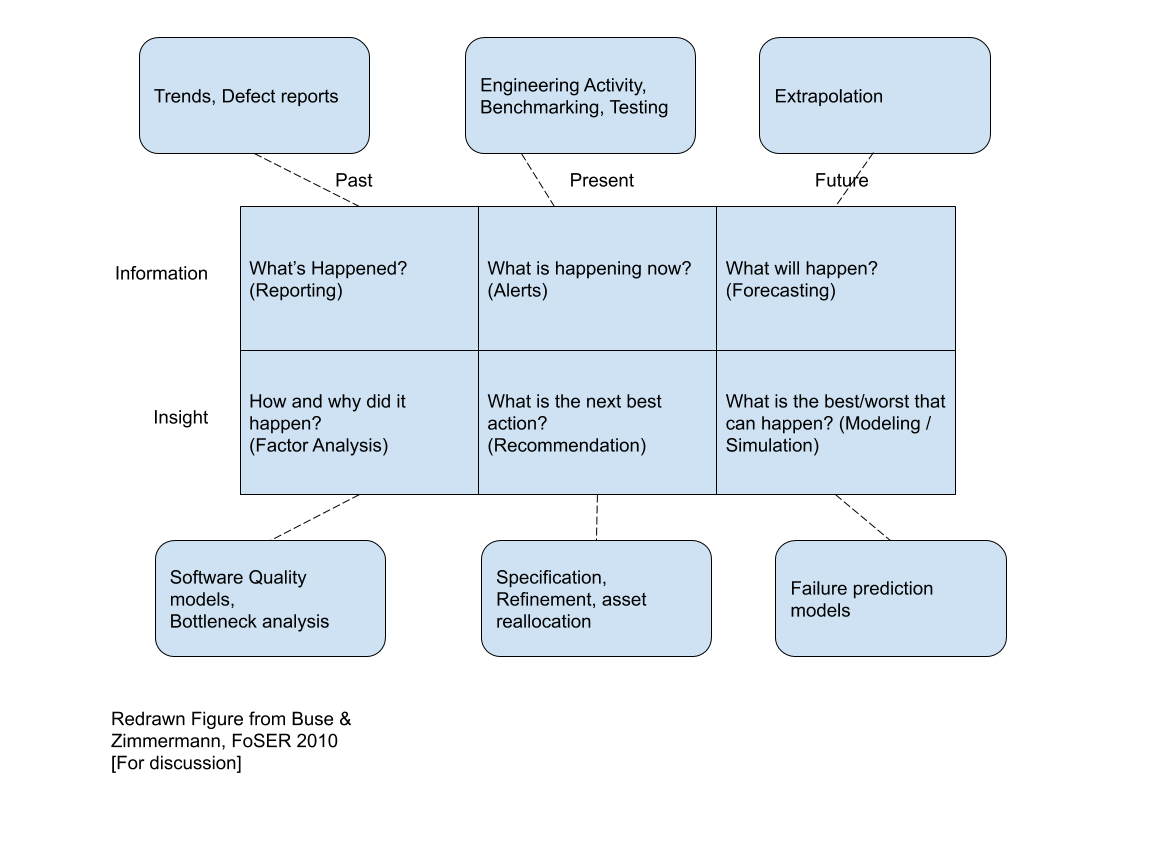
\includegraphics[width=\textwidth]{images/Buse_and_Zimmermann_2010_figure.png}
    \caption{Repeated here to map data sources to buckets}
    \label{fig:map_data_to_buckets}
\end{figure}

I aim to map various data sources (that originate from platform and app) in order to understand the effects of what we have done vs. understanding the practices and what users experience in order to improve our work and [thereby] the products we release.

\section{The platform and the app}
Mobile platform ecosystem 

\textbf{The platform as observer}: Google Android comprises of an operating system (Android), an app store (Google Play), various software installed on approved\footnote{and unapproved} Android certified devices, and related development tools and products provided by Google. \julian{How about I discuss platforms in general in a discussion chapter rather than here?}

\julian{Perhaps off topic or not sufficiently relevant for here: we could discuss how Google evolves and back-ports some of the evolution of Android across different releases of Android e.g. to enable some of the newer APIs and functionality to be available on older Android releases. Some of these seem to affect the data provided in Android Vitals for these older Android releases e.g. I cannot see any data, nor how to enable it for a test account on a device running Android KitKat (v4.4) and Google states some features are only available on Android 8.0 and newer releases (without providing any details)\cite{google_account_help_android_share_data_2019}}

Note: Users intended to be volunteers who offer their usage data for the good of the ecosystem.

\textbf{The app as a recorder and scribe}:

\chapter{Research Questions}
\textit{"How can app-centric data provide useful feedback that will guide the testing of mobile applications?"}
\julian{Discussion: how can I elegantly describe, label or name app-centric data in my research [and generally]?}

\todo{Define explicitly what app-centric data includes and what it excludes.}

c.f. pre- and post- treatment testing. e.g. perhaps you start without test cases, can app-centric data and my research help projects create some practical test cases?

\begin{outline}
  \1 How can the various data sources map to various aspects of testing of a mobile app? (c.f Buse and Zimmermann - place at end of literature review or in this chapter.)
    \2 What are the types of data sources available?
    \2 What are their strengths, weaknesses, opportunities, and threats for each type of data source? Also what are their range and scope?\footnote{This may be a chapter in my thesis, using the internal test app as the method. The method relevant to the sub-q can be embedded in the relevant chapter.}
      \3 How might these data sources be useful to measure aspects of the use of a mobile app? 
      \3 How might they be used to measure improvements in the product quality and/or product fit\footnote{product fit may consider the user's satisfaction of the product (the app) and its suitability for their purposes}?
        \4 Can we measure app quality using \textit{Relative Correctness} for releases of Android apps?
    \2 What does the Google Android ecosystem (\textit{A}ndroid \textit{G}oogle \textit{E}cosystem or \textit{AGE} for short?) provide in terms of data sources? (and why are these relevant to the research and the reader?)
      \3 What types of flaws can be measured? ANR's and crashes perhaps also proxy measures such as uninstalls and low usage of apps?
      \3 What can be determined of relevance in terms of the operational environment/envelope for Android apps? and how might these be relevant in terms of testing the app \textit{and} in terms of user experience \julian{This may be beyond the scope of my research...}? 
      \3 How trustworthy and complete are the tools provided in the Google Android ecosystem?
        \4 Do Crash Clusters in Android Vitals provide sufficient information to identify when the crash occurs? (rather than where in the code the crash occurs.) If not, what additional information would be relevant?
    \1 How can app-centric data provide useful/relevant\footnote{Can you test in a more targetted way, run fewer tests, ...? c.f. efficiency and effectiveness of testing and define these in turn.} feedback that will guide the testing of mobile applications?
      \2 How can app-centric data provide useful FEEDBACK on software testing of particular mobile apps? \julian{we can generalise the feedback from a particular app to provide guidance for the future testing of similar apps.}
      \2 How can app-centric data assist with the testing of mobile apps? (GUIDANCE). May also apply to similar apps. 
    \1 What is useful/relevant feedback for testing and how might we measure it?
  \1 Are the data only useful for testing aspects of mobile apps?
\end{outline}

\section{Answering the Research Questions using on Google Android ecosystem}
\subsection{Context}
Google provides various offerings either as distinct products or as part of the Google Play Console. These include Firebase\footnote{\url{https://developers.google.com/analytics/devguides/collection/firebase/android/}} and Crashlytics (which might be considered as products and/or services), and Google Play Console tools and reports, including: Android Vitals, Aquisition Reports, Release Management (including pre-launch reports), and User Feedback.

Broadly, the distinct products (Firebase and Crashlytics\footnote{There have been various acquisitions in terms of these types of products, Google now owns Fabric which owns Crashlytics - both of these are being subsumed into Firebase and are likely to replaced by similar offerings branded solely as Firebase. Currently (July 2019) Fabric still has independent branding, Crashlytics is documented both in Firebase and on fabric.io\url{https://docs.fabric.io/android/crashlytics/overview.html}}) can optionally be integrated by developers into one or more of their applications in order to collect details of how the applications are being used from \textit{[within] the perspective of the app}. 

Google Play Console's offerings provide ecosystem-level analytics. Some appear to be tracked by the app store (Google Play) directly (e.g. Installs/Uninstalls), others are recorded on end-user devices and only made available provided to the developer when various conditions have been met; \textit{i.e.} the users have opted-in to providing data from a particular device automatically \textit{and} various unpublished thresholds (set and used within Google's ecosystem) have been met.

How can the Google Android ecosystem (e.g. services, tools, and reports) provide useful feedback that will guide the testing of mobile applications?

What are the extents and limits of the Google Android ecosystem?

\subsection{Research Questions for Android Vitals}
\begin{itemize}
    \item What does Android Vitals offer to help provide feedback on the testing performed for a project's Android apps? \julian{Discuss how to identify and measure the testing we did using Android Vitals as the lens.}
    
    - Why focus on testing of [mobile| app store | \textbf{Android}] Apps? (the highest level motivation I have for this work). 

-- What difference can system level analytics make to the practice of testing?

-- What can operating system level analytics add to app level analytics? Explain what would need to exist for this to work. 
---- ANRs are unique to Android and need to be collected outside the app. Little research on ANRs. The app can't know it (Turing on non-determinism they cannot be detected by the algorithm and have to be detected externally e.g. by Android.)

-- Is testing the only thing you need to know about system level analytics? Firstly would this be of interest in terms of design, development, marketing? 

    \item (sub-question) What does Android Vitals provide that may help inspire refinements (e.g. operational envelope - device model, android release, locale setting, test duration, location, ...) to current tests and new tests? (Provide examples) 
    \julian{Some information may come from other parts of Google Play Console e.g. installs in various countries. Aims to discover more situations. c.f. refining requirements}
    - test generation, test coverage, regression test, etc. \textit{Why pick refinement, or is this a random choice?}
    
    \item Do Crash Clusters in Android Vitals provide sufficient information to identify when the crash occurs? (rather than where in the code the crash occurs.) If not, what additional information would be relevant? 
    \julian{A rich topic and one that may exemplify why Mobile Analytics is a useful ingredient in the mix.}
    - why are crashes important? They are important but not the only thing that's important for us. crashes are somewhat orthogonal to testing. why do we care about them in terms of this research and the larger practice. Acknowledge in the literature that lots of people worry about crashes. Make sure I explain that crashes aren't the only thing to worry about. Underlying hypothesis about user experience, and why crashes are relevant to the UX. UX is also orthogonal to testing. 
    - Venn diagram between ANRs \& crashes and user-experience, and perhaps testing. 
    
    \item Is the concept of relative correctness viable for Android apps? And can Android Vitals be used to measure relative correctness for releases of a given Android app? 
    
    - I need to explain relative correctness. (historical comparison across several releases of the software).
    
    \item What are the strengths and weaknesses of Android Vitals in relation to testing of the app being reported on? Are there sweetspots where Android Vitals is particularly useful for testing and quality improvement?
    
    - I'm already questioning the relevance of various areas of Android Vitals
    
    - This is more of experience report, collecting practices, engineering pains, etc. Interesting to highlight the underlying framework - something people didn't know before that I've explained. How can people improve the practice. The question is unclear so far.
    
    - The engineering of these tools vs the scientific aspects of the tools. Can I do a case study with and without Android Vitals for given apps? Can we control the experiment. Theoretical/conceptual input also useful. Classification of different properties of Android Vitals. Induce the theory from a number of instances, then find another instance and apply the theory. How could my theories be applied by others? Kiwix gave me the initial data, other apps provided additional colour and depth. Can this conceptional framework be applied to another app and lead to the same expected results i.e. is the work repeatable and generalisable? What we learn from m apps to apply to n apps. 
    
    - It's worth explaining the timeline of which apps have which tools in use in which order. Could we consider each release as a separate app? 
    
    - Forensics of the connections between ratings and crashes/ANRs; Forensics of the Testing. Prepare for forensic analysis and forensic readiness FSE 2017/8? Data needs to be long-lived, etc. c.f. Mobile Forensics. Civilian use of forensics. 
    
\end{itemize}

\subsection{Notes and guidance on the RQ's}

\subsubsection{An hourglass model}
An hourglass model to consider in my research design...

\begin{itemize}
    \item Start with the general (the top of the hourglass
    \item Exemplify with an instance of the general (e.g. Android Vitals, Crashlytics, ...)
    \item Assess how much of what we discover from the instance applies []back] to the general. (the bottom of the hourglass)
\end{itemize}

Can I generalise the tool in the Android Vitals section? Prerequisites to be able to use Android Vitals

- We can anonymise the role of who or what does the testing.

\yijun{Usually RQ's are nested or structured. Try to provide a clearly distinctive structure in the RQ's - makes the chapters easy to structure and to measure completeness, that they've all been answered. An iterative process to refine the questions with the answers.}


    1 formula saves 100 diagrams, 1 diagram saves 200 words. Aim for empirical formula. Empirical theory e.g. grounded theory: interviews. Action research rather than observational research.
    
    Good construct validity, but biases likely from my personal interests.  
    External validity may be weak. Ask for others to apply my ideas and interview them afterwards. OK to reflect on what I have done rather than doing new work, necessarily. Provide explanation, why didn't I find creative ways to overcome the challenges and blockers. 
    
    How did I achieve the goal (I still need to articulate the goal in my thesis). 
    
    If I discover things don't matter, by sharing this information it helps developers prioritise on other things that \textit{are important}. 
    
    Can I build a complementary story of what does matter? How can we capture the information that matters?
    
    For augmented stack traces discuss privacy management. 
    
    
\section{Example RQ's from other papers for comparison}

From \url{https://ieeexplore.ieee.org/abstract/document/8730164}
\begin{itemize}
    \item \textbf{RQ1} \textit{How do APR systems leverage FL techniques?} We first investigate FL techniques used in APR systems in the literature. This reveals which FL tool and formula are integrated for each APR system. We examine implementation details of each APR system, and/or directly ask the authors of the technique to clarify FL configuration, e.g., which level of detection granularity is considered, and how many suspicious locations are considered.
    \item \textbf{RQ2} \textit{How many bugs from a common APR benchmark are actually localizable?} After aggregating APR performance data reported in the literature, we note that 246 bugs (in benchmark Defects4J) have not yet been fixed by any state-of-the-art APR tool. Given that researchers scarcely discuss the reasons behind repair misses, we assess, with this research question, our intuition that FL is possibly one of the challenging steps in the repair pipeline.
    \item \textbf{RQ3} \textit{To what extent APR performance can vary by adapting different FL configurations?} We implement and make publicly available kPAR, a straightforward fix pattern-based APR system, and record its performance under various configurations to serve as a comparable baseline for future research.
\end{itemize}

I like their next section...
Eventually, we make the following contributions:

\begin{itemize}
    \item We expose a hidden bias throughout the comparison of APR tools in the literature, and present more reliable performance comparisons for current state-of-the-art.
    \item We build and make publicly available an easy-to-configure fault localization toolkit that can be adopted in APR pipelines for Java programs.
    \item We provide a refined benchmark for evaluating the performance of APR systems with respect to those bugs that can actually be localized.
    \item We implement and make publicly available a baseline APR system with its different performance metrics for different FL configurations.
    \item Our replication package, including kPAR, is available at: \url{https://github.com/SerVal-DTF/FL-VS-APR}
\end{itemize}



